% arXiv preprint format
% Primary: cs.SE (Software Engineering)
% Secondary: cs.AI (Artificial Intelligence), cs.MA (Multi-Agent Systems)
\documentclass[11pt,a4paper]{article}

\usepackage[margin=1in]{geometry}
\usepackage{amsmath,amssymb,amsfonts}
\usepackage{algorithmic}
\usepackage{graphicx}
\usepackage{textcomp}
\usepackage{xcolor}
\usepackage{booktabs}
\usepackage[colorlinks=true,linkcolor=blue,citecolor=blue,urlcolor=blue]{hyperref}
\usepackage{multirow}
\usepackage{array}
\usepackage{listings}
\usepackage{tabularx}
\usepackage{enumitem}
\usepackage{tikz}
\usepackage{authblk}
% Using thebibliography directly; switch to .bib + natbib for full arXiv pipeline
\usetikzlibrary{shapes.geometric, arrows.meta, positioning, fit, backgrounds}

\lstset{
  basicstyle=\ttfamily\footnotesize,
  breaklines=true,
  frame=single,
  columns=fullflexible,
  keepspaces=true,
  showstringspaces=false,
  commentstyle=\color{gray},
  keywordstyle=\color{blue},
  stringstyle=\color{red}
}

\begin{document}

\title{One Human, Sixteen Agents:\\ Building Production Software with Role-Specialized LLM Pipelines}

\author[1]{Najwa Alghamdi}
\affil[1]{Independent Researcher / Founder\\ \texttt{Research@Najwa.io}}

\date{March 2026}

\maketitle

\begin{abstract}
Most AI-assisted development treats LLMs as tools that help developers write code faster---the developer still architects, reviews, tests, and secures the code themselves. This paper argues for a different framing: LLMs as a \textit{team} that enables engineering processes a solo developer would otherwise routinely skip. We decompose the SDLC into 16 role-specialized agents with enforced tool access, domain-embedded prompts, and structured output schemas, and deploy the pipeline over 11 sprints to build a production multi-tenant SaaS platform. Four findings stand out. \textbf{First}, multi-agent role separation enables quality processes---independent review, adversarial testing, dual-perspective validation---that monolithic AI assistance cannot replicate effectively, because a single session playing every role suffers from role contamination, blind spot persistence, and permission overreach. \textbf{Second}, runtime tool restriction produces qualitatively different agent behavior: a reviewer with edit access physically removed generates 3--5$\times$ longer explanations with file-line references and severity justifications than one merely instructed not to edit---demonstrating that capability restriction, not prompt engineering, enforces role boundaries. \textbf{Third}, dual independent reviews using different models (Opus vs.\ Sonnet+Codex) achieve only 32.8\% issue overlap ($n=125$, 8{,}970 LOC), with the \textit{cheaper} pairing finding $2\times$ more exclusive issues including all exclusive CRITICALs---suggesting model diversity matters more than model size. \textbf{Fourth}, a dedicated red team agent found 8 exploitable vulnerabilities in code that had passed four prior quality stages, including a critical unauthenticated admin API---confirming that adversarial testing catches what standard quality gates systematically miss. None of these gains required a more powerful model; they emerged from process architecture. We introduce cross-model composition (Claude+OpenAI for review, Claude+Gemini for UI validation) and distill seven design principles for practitioners.
\end{abstract}

\noindent\textbf{Keywords:} Large Language Models, Multi-Agent Systems, Software Development Life Cycle, Role Specialization, Tool-Use Agents, Code Review Automation, Adversarial Testing, Human-in-the-Loop, Cross-Model Validation

%% ============================================================
\section{Introduction}

\subsection{Motivation}

Large Language Models have become ubiquitous software development assistants, with tools such as GitHub Copilot, Cursor, and Claude Code seeing rapid adoption since 2023. Yet the dominant interaction paradigm treats AI as a \textbf{tool}---a faster way to write code, with a single LLM session serving identical context, identical permissions, and identical expertise across all phases. The human operator remains solely responsible for architectural decisions, quality judgment, and security assurance. For solo developers and small teams, this means that essential quality gates---independent code review, adversarial security testing, structured QA---are simply skipped. Not because developers are careless, but because one person cannot meaningfully review their own code, attack their own system, or test against acceptance criteria they themselves wrote.

This paper asks a different question: \textit{what if AI served not as a tool that helps you code faster, but as a team that lets you run processes you otherwise couldn't?} Rather than using one powerful model to generate more code, we decompose the SDLC into 16 role-specialized agents---each with constrained capabilities, distinct expertise, and structured outputs---enabling a solo developer to consistently run independent review, adversarial testing, and multi-stage quality gates that would otherwise be routinely skipped.

The monolithic paradigm that we replace suffers from several well-documented limitations:

\begin{enumerate}
    \item \textbf{Role contamination}---An agent that just wrote code is poorly positioned to objectively review it~\cite{beller2014}. Cognitive anchoring on one's own implementation reduces the likelihood of identifying architectural issues or alternative approaches.
    \item \textbf{Blind spot persistence}---A single model's systematic biases apply uniformly across all development phases. If the model tends to overlook certain vulnerability classes, that blind spot persists from design through deployment.
    \item \textbf{Permission overreach}---An assistant with write access may ``helpfully'' fix issues rather than articulating them, reducing feedback quality. We demonstrate empirically that this behavioral shift is measurable (Section~\ref{sec:rq1}).
    \item \textbf{Domain knowledge dilution}---A generic system prompt cannot encode deep domain-specific checklists, compliance rules, locale-specific business logic, and edge cases simultaneously for all SDLC phases.
    \item \textbf{Context window saturation}---A monolithic session accumulating design documents, implementation code, review feedback, and test results risks exceeding context limits or degrading reasoning quality through attention dilution.
\end{enumerate}

Human engineering organizations solved these problems long ago through role specialization: architects design, developers implement, reviewers review (with read-only repository access in many organizations), QA engineers test against acceptance criteria, and security teams conduct adversarial assessments. Each role has distinct permissions, distinct expertise, and distinct output expectations. Our thesis is that \textbf{process architecture matters more than model capability}---the quality gains in this study come not from using a smarter model, but from structuring how multiple models interact through enforced roles, constrained capabilities, and adversarial stages.

\subsection{Research Questions}

This study investigates:

\begin{itemize}[leftmargin=*]
    \item \textbf{RQ1:} Does runtime tool-scoping (enforced capability restriction) produce qualitatively different agent behavior compared to prompt-based instruction alone?
    \item \textbf{RQ2:} Do dual independent LLM-based code reviews---using different models and augmentation tools---provide complementary or redundant coverage, and does cross-model composition (Opus vs.\ Sonnet+Codex) yield distinct specialization?
    \item \textbf{RQ3:} Can an embedded red team agent identify security vulnerabilities that survive the standard design $\rightarrow$ implement $\rightarrow$ review $\rightarrow$ test pipeline?
    \item \textbf{RQ4:} What are the practical utilization patterns, failure modes, and cost characteristics of a 16-agent SDLC pipeline over multiple sprints?
\end{itemize}

\subsection{Contributions}

\begin{enumerate}
    \item A detailed architecture for decomposing the SDLC into 16 role-specialized LLM subagents with enforced tool scoping, including a formal tool access matrix and system prompt taxonomy.
    \item Empirical data from 11 production sprints, including dual-review overlap analysis ($n=125$ issues across 8{,}970 LOC), red team attack results ($n=30$ attacks), conversation-level test outcomes ($n=858$ checks), and sprint-by-sprint shipping velocity.
    \item A cross-model review methodology pairing Opus with Sonnet+Codex, revealing that model diversity drives complementary coverage (32.8\% overlap)---with Sonnet+Codex excelling at security and Opus at architecture. Additionally, Claude + Gemini composition for UI validation.
    \item A conversation testing framework (\texttt{conv-sim}) with 6 personas, 13 scenarios, and 11 automated bug detectors for evaluating conversational AI quality.
    \item Seven design principles and four anti-patterns for multi-agent development pipelines, derived from 11 sprints of practitioner experience.
\end{enumerate}

%% ============================================================
\section{Related Work}

\subsection{LLMs for Software Engineering}

Recent work has demonstrated LLM effectiveness across individual SDLC phases: code generation~\cite{chen2021, li2023starcoder}, code review~\cite{li2022, tufano2022}, test generation~\cite{lemieux2023}, and vulnerability detection~\cite{pearce2023}. However, these studies typically evaluate models in isolation on single tasks, rather than as coordinated multi-agent pipelines operating over sustained development periods.

SWE-bench~\cite{jimenez2024} and similar benchmarks evaluate LLMs on isolated bug fixes. SWE-agent~\cite{yang2024} and OpenHands~\cite{wang2024openhands} build agent-computer interfaces that can resolve SWE-bench issues autonomously, while MapCoder~\cite{islam2024} decomposes competitive programming into multi-agent pipelines. Liu et al.~\cite{liu2024survey} provide a comprehensive survey of LLM-based agents for software engineering. However, none assess the multi-phase SDLC workflow (design $\rightarrow$ implement $\rightarrow$ review $\rightarrow$ test $\rightarrow$ secure) that characterizes real software development over sustained periods.

\subsection{Multi-Agent LLM Systems}

Multi-agent frameworks such as AutoGen~\cite{wu2023}, MetaGPT~\cite{hong2023}, and ChatDev~\cite{qian2023} have explored role-based agent decomposition for software tasks. MetaGPT assigns roles (Product Manager, Architect, Engineer) and enforces Standardized Operating Procedures (SOPs) between agents. ChatDev simulates a software company with CEO, CTO, Programmer, and Tester roles. AgentCoder~\cite{huang2024} decomposes code generation into programmer, test designer, and test executor agents.

Our work differs in four key ways:

\begin{enumerate}
    \item \textbf{Production deployment}---unlike simulated or benchmark environments, our pipeline was used to build a real, multi-tenant production system over 11 sprints, with shipping deadlines and compliance requirements.
    \item \textbf{Enforced tool scoping}---prior work relies on prompt-based role adherence; we enforce constraints at the runtime level via tool whitelisting, demonstrating a measurable behavioral difference (Section~\ref{sec:rq1}).
    \item \textbf{Adversarial agents}---we include dedicated red team and dual-review agents, absent from prior multi-agent SDLC frameworks.
    \item \textbf{Cross-model composition}---individual agents combine outputs from multiple LLM providers (Claude + OpenAI for code review; Claude + Gemini for UI validation), extending tool-augmented LLM patterns~\cite{schick2023} to cross-provider validation.
\end{enumerate}

\subsection{LLM-Based Code Review}

Fan et al.~\cite{lu2023} surveyed automated code review with LLMs, finding that models can identify functional bugs, security issues, and style violations, but struggle with deep architectural reasoning and domain-specific compliance. Li et al.~\cite{li2022} demonstrated pre-trained models for code review activities, achieving improvements over template-based approaches. Our work extends this by: (a)~embedding domain-specific checklists directly into reviewer system prompts; (b)~measuring dual-review overlap rates with differentiated review focus; and (c)~combining two competing LLM providers for cross-validation.

\subsection{Adversarial Testing of LLM Applications}

Prompt injection attacks~\cite{perez2022, greshake2023} and LLM application vulnerabilities~\cite{owasp2025} have been extensively documented. Deng et al.~\cite{deng2024} proposed systematic red-teaming frameworks for LLM applications. However, embedding adversarial testing as a \textit{standard SDLC phase}---with a dedicated agent that attacks every feature before release, using a structured 7-category attack playbook---is, to our knowledge, novel in practice.

\subsection{Domain-Specific LLM Customization}

Prior work on domain adaptation for LLMs has focused on fine-tuning~\cite{gururangan2020} or retrieval-augmented generation~\cite{lewis2020}. Our approach---embedding domain knowledge directly in system prompts (100+ lines per agent)---represents a zero-training-cost alternative that functions as persistent institutional memory across sessions.

%% ============================================================
\section{System Architecture}

\subsection{Framework Overview}

The system is built on Claude Code's \texttt{.claude/agents/} framework, which allows definition of subagents via markdown files with YAML frontmatter. Each agent definition specifies:

\begin{lstlisting}[language=yaml, caption={Agent definition schema}]
---
name: <identifier>
description: <natural language description>
tools: <comma-separated tool whitelist>
model: <opus | sonnet | haiku>
---
<system prompt body: 50-200 lines>
\end{lstlisting}

The runtime enforces the \texttt{tools} whitelist at the infrastructure level: an agent defined with \texttt{tools: Read, Glob, Grep, Bash} physically cannot invoke \texttt{Edit} or \texttt{Write} operations, regardless of what the system prompt instructs or what the model attempts. This is a critical distinction from prompt-based constraints, which rely on the model's compliance and are susceptible to jailbreaking or instruction drift.

\subsection{Available Tools}

Table~\ref{tab:tools} enumerates the tool primitives available for agent assignment.

\begin{table}[htbp]
\caption{Available Tool Primitives}
\label{tab:tools}
\centering
\footnotesize
\begin{tabular}{@{}llp{3.5cm}@{}}
\toprule
\textbf{Tool} & \textbf{Category} & \textbf{Description} \\
\midrule
Read & File I/O & Read file contents \\
Glob & Search & Find files by pattern \\
Grep & Search & Search file contents (regex) \\
Bash & Execution & Execute shell commands \\
Edit & File I/O & Modify existing files \\
Write & File I/O & Create/overwrite files \\
Agent & Orchestration & Spawn child subagents \\
WebSearch & Network & Search the web \\
WebFetch & Network & Fetch URL contents \\
MCP* & Extension & Model Context Protocol tools (OpenAI, Gemini) \\
\bottomrule
\multicolumn{3}{l}{\footnotesize *MCP tools provide cross-model access via protocol.}
\end{tabular}
\end{table}

\subsection{Agent Taxonomy}
\label{sec:taxonomy}

We define 16 agents organized into a pre-ops pipeline (12 agents) and an ops team (4 agents). Tables~\ref{tab:preops} and~\ref{tab:ops} detail the full taxonomy.

\begin{table}[htbp]
\caption{Pre-Ops Pipeline Agents (12 agents)}
\label{tab:preops}
\centering
\footnotesize
\begin{tabular}{@{}llcccc@{}}
\toprule
\textbf{Name} & \textbf{Role} & \textbf{Model} & \textbf{Edit} & \textbf{Web} & \textbf{Lines} \\
\midrule
Tariq & Product Owner & Opus & -- & \checkmark & 73 \\
Dana & UX Researcher & Sonnet & -- & \checkmark & 60 \\
Lina & UI Designer$^\ddagger$ & Opus & \checkmark & -- & 144 \\
Faisal & Architect & Opus & -- & -- & 104 \\
Rania & Developer & Opus & \checkmark & -- & 81 \\
Khaled & Reviewer 1 & Opus & \textbf{--} & -- & 104 \\
Nasser & Reviewer 2$^\dagger$ & Sonnet+Codex & \textbf{--} & -- & 100 \\
Layla & QA Engineer & Opus & \checkmark & -- & 112 \\
Youssef & Prompt Tester & Opus & \checkmark & -- & 122 \\
Huda & Conv. Tester & Opus & \checkmark & -- & 142 \\
Zaid & Red Team & Opus & \checkmark & -- & 203 \\
Maha & Doc Writer & Sonnet & \checkmark & -- & 50 \\
\bottomrule
\multicolumn{6}{l}{\footnotesize $^\dagger$ OpenAI Codex access via MCP. $^\ddagger$ Gemini access via MCP.}
\end{tabular}
\end{table}

\begin{table}[htbp]
\caption{Ops Team Agents (4 agents)}
\label{tab:ops}
\centering
\footnotesize
\begin{tabular}{@{}llccc@{}}
\toprule
\textbf{Name} & \textbf{Role} & \textbf{Model} & \textbf{Edit} & \textbf{Lines} \\
\midrule
Sultan & DevOps & Opus & \checkmark & 100 \\
Aws & SRE & Opus & \checkmark & 133 \\
Majid & Database Admin & Sonnet & \checkmark & 131 \\
Reema & Analytics & Sonnet & \checkmark & 143 \\
\bottomrule
\end{tabular}
\end{table}

\textbf{Total system prompt volume:} $\sim$1,800 lines across 16 agents, comprising approximately 45,000 tokens of domain knowledge, checklists, output templates, and behavioral instructions.

\subsection{Tool Scoping as Access Control}
\label{sec:toolscoping}

A central design principle is that \textbf{tool scoping enforces role boundaries more reliably than prompt instruction}. Table~\ref{tab:toolmatrix} illustrates the access control matrix across role categories.

\begin{table}[htbp]
\caption{Tool Access Matrix by Role Category}
\label{tab:toolmatrix}
\centering
\footnotesize
\begin{tabular}{@{}lccccccc@{}}
\toprule
\textbf{Capability} & \textbf{PO} & \textbf{Arch} & \textbf{Dev} & \textbf{Rev} & \textbf{QA} & \textbf{Red} & \textbf{Ops} \\
\midrule
Read files & \checkmark & \checkmark & \checkmark & \checkmark & \checkmark & \checkmark & \checkmark \\
Search code & \checkmark & \checkmark & \checkmark & \checkmark & \checkmark & \checkmark & \checkmark \\
Shell exec & \checkmark & \checkmark & \checkmark & \checkmark & \checkmark & \checkmark & \checkmark \\
Edit files & -- & -- & \checkmark & \textbf{--} & \checkmark & \checkmark & \checkmark \\
Write files & -- & -- & \checkmark & \textbf{--} & \checkmark & \checkmark & \checkmark \\
Spawn agents & -- & \checkmark & \checkmark & -- & \checkmark & -- & -- \\
Web access & \checkmark & -- & -- & -- & -- & -- & -- \\
Cross-model & -- & -- & -- & R2 & -- & -- & -- \\
\bottomrule
\end{tabular}
\end{table}

The design encodes several deliberate constraints:

\begin{itemize}[leftmargin=*]
    \item \textbf{Reviewers cannot edit.} This forces articulate, explanatory feedback rather than quick patches (Section~\ref{sec:rq1}).
    \item \textbf{Architects cannot write code.} This ensures architectural output remains at the design level---data models, API contracts, tool schemas---not implementation.
    \item \textbf{Product Owner has web access.} The PO can research market requirements, competitor features, and regulatory updates---capabilities irrelevant to other roles.
    \item \textbf{Only 3 roles can spawn child agents.} Architect, Developer, and QA can delegate subtasks; other roles are terminal executors.
\end{itemize}

\subsection{System Prompt Architecture}
\label{sec:promptarch}

Each agent's system prompt follows a six-layer structure. We formalize this as the \textbf{IRDCOP} framework:

\begin{enumerate}
    \item \textbf{I}dentity---Role definition, persona name, reporting line, organizational position.
    \item \textbf{R}esponsibilities---Enumerated duties (5--8 items per agent).
    \item \textbf{D}omain knowledge---Technology stack references, data model paths, compliance rules, locale-specific business logic, known edge cases.
    \item \textbf{C}ross-references---Explicit pointers to other agents' outputs, contracts, and shared artifacts.
    \item \textbf{O}utput format---Structured schemas (tables, checklists, verdict formats, severity classifications) that standardize agent output for downstream consumption.
    \item \textbf{P}rinciples---Design principles, anti-patterns, and behavioral constraints.
\end{enumerate}

In our case, the target domain involves locale-specific regulations, bilingual requirements, multi-tenant data isolation, and compliance rules---each embedded across the relevant agents. The key insight is that domain rules written once are automatically loaded into every future agent invocation, creating a compounding return on prompt engineering investment.

\subsection{Cross-Model Agent Composition}
\label{sec:crossmodel}

Two agents in our taxonomy access competing LLM providers via the Model Context Protocol (MCP):

\textbf{Nasser (Reviewer~2)} is powered by Claude Sonnet but has access to OpenAI Codex via two MCP tools:
\begin{itemize}[leftmargin=*]
    \item \texttt{codex\_review}---Sends code to OpenAI for independent review.
    \item \texttt{codex\_suggest\_fix}---Sends problematic code for alternative fix suggestions.
\end{itemize}

\textbf{Lina (UI Designer)} is powered by Claude Opus but has access to Google Gemini via two MCP tools:
\begin{itemize}[leftmargin=*]
    \item \texttt{gemini\_review\_ui}---Sends HTML/CSS to Gemini for UI/UX review (accessibility, responsive, RTL, visual hierarchy).
    \item \texttt{gemini\_suggest\_ui}---Asks Gemini for alternative component designs or HTML/CSS prototypes.
\end{itemize}

This cross-model composition creates agents that combine the reasoning strengths of multiple providers. We hypothesize that each LLM has different systematic biases, and cross-validation exposes issues that any single model might miss (Section~\ref{sec:rq2}).

\subsection{Pipeline Orchestration}
\label{sec:pipeline}

The agents are organized into a five-phase sequential pipeline with a human orchestrator:

\begin{figure}[htbp]
\centering
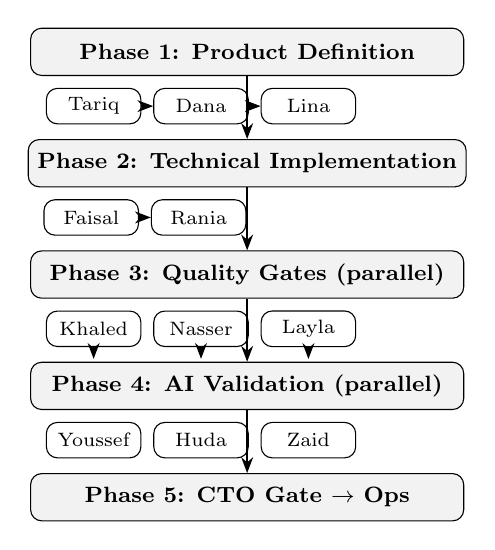
\begin{tikzpicture}[
    node distance=0.4cm and 0.6cm,
    phase/.style={draw, rounded corners, minimum width=5.5cm, minimum height=0.6cm, font=\footnotesize\bfseries, fill=gray!10},
    agent/.style={draw, rounded corners, minimum width=1.2cm, minimum height=0.45cm, font=\scriptsize, fill=white},
    arr/.style={-{Stealth[length=2mm]}, thick},
    parr/.style={-{Stealth[length=2mm]}, thick, dashed}
]
% Phases
\node[phase] (p1) {Phase 1: Product Definition};
\node[phase, below=0.8cm of p1] (p2) {Phase 2: Technical Implementation};
\node[phase, below=0.8cm of p2] (p3) {Phase 3: Quality Gates (parallel)};
\node[phase, below=0.8cm of p3] (p4) {Phase 4: AI Validation (parallel)};
\node[phase, below=0.8cm of p4] (p5) {Phase 5: CTO Gate $\rightarrow$ Ops};

% Agents per phase (positioned between phase boxes)
\node[agent, below=0.15cm of p1.south west, anchor=north west, xshift=0.2cm] (tariq) {Tariq};
\node[agent, right=0.15cm of tariq] (dana) {Dana};
\node[agent, right=0.15cm of dana] (lina) {Lina};

\node[agent, below=0.15cm of p2.south west, anchor=north west, xshift=0.2cm] (faisal) {Faisal};
\node[agent, right=0.15cm of faisal] (rania) {Rania};

\node[agent, below=0.15cm of p3.south west, anchor=north west, xshift=0.2cm] (khaled) {Khaled};
\node[agent, right=0.15cm of khaled] (nasser) {Nasser};
\node[agent, right=0.15cm of nasser] (layla) {Layla};

\node[agent, below=0.15cm of p4.south west, anchor=north west, xshift=0.2cm] (youssef) {Youssef};
\node[agent, right=0.15cm of youssef] (huda) {Huda};
\node[agent, right=0.15cm of huda] (zaid) {Zaid};

% Arrows between phases
\draw[arr] (p1.south) -- (p2.north);
\draw[arr] (p2.south) -- (p3.north);
\draw[arr] (p3.south) -- (p4.north);
\draw[arr] (p4.south) -- (p5.north);

% Sequential arrows within phases
\draw[arr] (tariq) -- (dana);
\draw[arr] (dana) -- (lina);
\draw[arr] (faisal) -- (rania);

% Parallel indicators
\draw[parr] (khaled.south) -- ++(0,-0.15);
\draw[parr] (nasser.south) -- ++(0,-0.15);
\draw[parr] (layla.south) -- ++(0,-0.15);

\end{tikzpicture}
\caption{Five-phase pipeline with human orchestrator between phases. Solid arrows = sequential. Dashed arrows = parallelizable.}
\label{fig:pipeline}
\end{figure}

The human operator serves as orchestrator between phases: invoking agents, passing context, and making gate decisions (``proceed,'' ``rework,'' or ``defer''). Within Phases~3 and~4, agents operate on the same codebase independently and can execute in parallel, reducing wall-clock time from $3\times$ to approximately $1\times$ without reducing coverage.

\subsection{Conversation Testing Framework}
\label{sec:convsim}

We developed a custom conversation testing library (\texttt{conv-sim}) that operates as an automated QA harness for conversational AI agents. The framework comprises four components:

\textbf{Personas} ($n=6$): Each persona has a fixed user ID, language preference, role, and behavioral profile:
\begin{itemize}[leftmargin=*]
    \item \textit{Persona~1} (Arabic, senior role)---tests standard workflow requests
    \item \textit{Persona~2} (Arabic, new user)---tests basic flows, escalation
    \item \textit{Persona~3} (Arabic, manager)---tests policy-heavy workflows
    \item \textit{Persona~4} (Arabic, technical role)---tests cross-agent routing
    \item \textit{Persona~5} (English, non-native speaker)---tests English-language flows
    \item \textit{Adversarial} (mixed)---tests prompt injection, gibberish, contradictions
\end{itemize}

\textbf{Scenarios} ($n=13$): Multi-turn conversation scripts covering: happy-path workflow, insufficient resource, duplicate detection, natural date parsing, status check, policy-specific workflow, policy questions, team-level queries, escalation, adversarial attacks, holiday-spanning requests, cancellation flow, and cross-agent routing.

\textbf{Bug Detectors} ($n=11$): Automated checks executed on every conversation turn:
\begin{enumerate}[leftmargin=*]
    \item \texttt{language\_consistency}---Response language matches persona preference
    \item \texttt{no\_raw\_enum}---No internal enum values (e.g., \texttt{Status.value}) leaking into user-facing text
    \item \texttt{response\_not\_empty}---Non-empty response body
    \item \texttt{no\_500\_error}---No server errors
    \item \texttt{correct\_agent}---Correct agent handled the request
    \item \texttt{response\_contains\_date}---Dates present when expected
    \item \texttt{mentions\_quota}---Relevant quota or entitlement figures mentioned when expected
    \item \texttt{detects\_duplicate}---Overlap or conflict detected when expected
    \item \texttt{mentions\_escalation}---Escalation to human offered when expected
    \item \texttt{mentions\_calendar\_conflict}---Calendar or scheduling conflict noted when request spans one
    \item \texttt{latency}---Response under 10 seconds
\end{enumerate}

\textbf{Reporter}: Produces terminal summary and JSON report with per-turn, per-detector pass/fail data.

All tests execute via real HTTP requests against the running application---not mocks---ensuring end-to-end validation including database state, LLM responses, and tool execution.

%% ============================================================
\section{Methodology}

\subsection{Study Context}

The pipeline was used to build a production multi-tenant B2B SaaS platform targeting Saudi Arabia. The platform serves multiple conversational AI agents behind a shared chat interface, each operating over the same multi-tenant data layer. The domain involves structured workflows, government compliance rules, and bilingual user interactions---characteristics that stress-test agent specialization, access control, and locale-aware generation. Table~\ref{tab:techprofile} summarizes the technical profile.

\begin{table}[htbp]
\caption{Platform Technical Profile}
\label{tab:techprofile}
\centering
\footnotesize
\begin{tabular}{@{}ll@{}}
\toprule
\textbf{Dimension} & \textbf{Value} \\
\midrule
Stack & Python 3.12, FastAPI, async SQLAlchemy 2.0 \\
Database & PostgreSQL + pgvector (1536-dim embeddings) \\
AI layer & Claude (claude-sonnet-4-6), tool-use loops (max 5 rounds/turn) \\
Tenancy & Row-level isolation (\texttt{tenant\_id}), JWT auth, Redis queuing \\
Locale & Bilingual (Arabic/English), Saudi regulatory compliance \\
Scale & 22 tables, 123 API endpoints, $\sim$40K LOC, 126 tests \\
Frontend & Self-contained HTML/CSS/JS (no build toolchain) \\
\bottomrule
\end{tabular}
\end{table}

\subsection{Study Duration and Sprint Structure}

Eleven development sprints conducted between February and March 2026 by a single developer. Each sprint followed the five-phase pipeline (Figure~\ref{fig:pipeline}). Table~\ref{tab:sprintplan} summarizes sprint deliverables.

\begin{table}[htbp]
\caption{Sprint Plan and Deliverables}
\label{tab:sprintplan}
\centering
\footnotesize
\begin{tabular}{@{}clp{5cm}c@{}}
\toprule
\textbf{Sprint} & \textbf{Focus} & \textbf{Deliverable} & \textbf{Tools} \\
\midrule
1--2 & Foundation & Core platform, Agent~A, RAG pipeline, chat UI & 19 \\
3--6 & Agent~B & Multi-step workflows, cross-agent routing, security hardening & 14 \\
7 & Agent~C M1 & Domain pipeline, AI-assisted content generation, web search & 13 \\
8 & Agent~C M2 & Interactive AI workflows, structured assessments & 8 \\
9 & Agent~C M3 & Cross-module analysis and decision support & 7 \\
10 & Agent~D & Operational intelligence, compliance monitoring, agent factory & 17 \\
11 & Agent~E & Executive analytics and compliance dashboards & 7 \\
\bottomrule
\end{tabular}
\end{table}

\subsection{Data Collection}

We collected five categories of data:

\begin{enumerate}[leftmargin=*]
    \item \textbf{Agent invocation logs}---Which agents were invoked per sprint, frequency, output size, and session duration.
    \item \textbf{Code review findings}---Issues identified by Khaled (Reviewer~1) and Nasser (Reviewer~2) independently, categorized by severity, type, and which reviewer found them.
    \item \textbf{Red team results}---Attack scenarios attempted, outcomes (blocked/succeeded/partial), severity classification, and post-fix verification.
    \item \textbf{Conversation test results}---\texttt{conv-sim} JSON reports with per-turn, per-detector pass/fail data.
    \item \textbf{Shipping metrics}---Tools implemented per agent, sprints to completion, pipeline passes, review rounds required.
\end{enumerate}

\subsection{Dual-Review Protocol}
\label{sec:dualprotocol}

For each major feature, both Khaled (Reviewer~1) and Nasser (Reviewer~2) independently review the same code. The protocol enforces:

\begin{itemize}[leftmargin=*]
    \item \textbf{Blind independence}---Nasser does \textit{not} see Khaled's review output.
    \item \textbf{Differentiated focus}---Khaled's prompt (Claude Opus) emphasizes architectural compliance, pattern consistency, and performance (N+1 queries, blocking I/O). Nasser's prompt (Claude Sonnet + OpenAI Codex via MCP) emphasizes edge cases, race conditions, null paths, incomplete rollback, and Arabic text handling.
    \item \textbf{Cross-model validation}---Nasser additionally consults OpenAI Codex via MCP tools (\texttt{codex\_review}, \texttt{codex\_suggest\_fix}), combining Claude Sonnet's analysis with OpenAI's independent perspective.
    \item \textbf{Structured output}---Both produce verdicts (APPROVE / REQUEST CHANGES) with tabular issue listings including file:line references and severity classifications.
\end{itemize}

Issues are classified post-hoc into three categories: found by Khaled only, found by Nasser only, or found by both (overlap).

\subsection{Red Team Protocol}
\label{sec:redprotocol}

Zaid (Red Team agent) operates with a 203-line system prompt---the longest in the taxonomy---containing a structured attack playbook across 7 categories:

\begin{enumerate}[leftmargin=*]
    \item \textbf{Prompt injection} (5 subcategories)---Direct override, delimiter escape, indirect injection via tool results, role confusion, multi-turn manipulation.
    \item \textbf{Data exfiltration} (3 subcategories)---Cross-user access, user enumeration, system prompt extraction.
    \item \textbf{Privilege escalation} (3 subcategories)---Admin API without auth, self-approval via agent, balance manipulation.
    \item \textbf{Tenant boundary violation} (2 subcategories)---Cross-tenant data access via API and via agent.
    \item \textbf{PII leakage}---Sensitive data in error messages, logs, or responses. Targets: government ID (Critical), salary (Critical), compliance status (High), contact information (High).
    \item \textbf{API security} (3 subcategories)---IDOR, mass assignment, rate limiting.
    \item \textbf{Abuse scenarios} (3 subcategories)---Balance drain via mass submit/cancel, conversation flooding, malicious content injection (XSS, template injection).
\end{enumerate}

The red team agent is invoked \textit{only after} the standard pipeline (design $\rightarrow$ implement $\rightarrow$ review $\rightarrow$ QA) is complete, simulating an external attacker encountering the ``finished'' product.

\subsection{Prompt Testing Protocol}

Youssef (Prompt Tester) evaluates the AI layer across 6 test categories:

\begin{enumerate}[leftmargin=*]
    \item \textbf{Tool selection}---Correct tool called for each intent (12 test cases, Arabic + English).
    \item \textbf{Parameter extraction}---Correct parameters from natural language (dates, entity types, identifiers).
    \item \textbf{Hallucination detection}---Agent must never invent data, policies, or balances.
    \item \textbf{Boundary testing}---Agent stays in scope (domain-specific agent refuses out-of-scope queries).
    \item \textbf{Bilingual equivalence}---Same question in Arabic and English produces equivalent answers (same numbers, same dates).
    \item \textbf{Edge cases}---Empty input, single-word confirmations, gibberish, mixed AR/EN, very long messages.
\end{enumerate}

All tests run via the actual chat API (\texttt{POST /api/v1/chat}), not by calling tools directly, ensuring the full agent loop (system prompt $\rightarrow$ tool selection $\rightarrow$ tool execution $\rightarrow$ response generation) is exercised.

%% ============================================================
\section{Results}

The core question underlying this study is whether a multi-agent pipeline with enforced role separation produces measurably different outcomes than monolithic AI assistance, where a single LLM session handles all SDLC phases with identical permissions and context. The results below address this question across four dimensions: behavioral differences from capability restriction (RQ1), coverage gains from independent review (RQ2), vulnerabilities caught only by adversarial testing (RQ3), and practical utilization patterns (RQ4).

\subsection{RQ1: Monolithic vs.\ Role-Separated Agent Behavior}
\label{sec:rq1}

In a monolithic workflow, a single LLM session with full tool access (Read, Write, Edit, Bash) performs both implementation and review. To measure how this compares to a role-separated agent, we tested the same reviewer model under two configurations: (a)~\textbf{monolithic-style}---all tools available, with a prompt instruction to ``review only, do not edit files''; and (b)~\textbf{role-separated}---Edit/Write tools physically removed from the agent's tool whitelist. Table~\ref{tab:scopingcomparison} summarizes the results.

\begin{table}[htbp]
\caption{Monolithic-Style vs.\ Role-Separated Agent Comparison}
\label{tab:scopingcomparison}
\centering
\footnotesize
\begin{tabular}{@{}lcc@{}}
\toprule
\textbf{Metric} & \textbf{Monolithic} & \textbf{Role-Separated} \\
\midrule
Edit attempts & $\sim$15\% & 0\% \\
Avg sentences per issue & 1--2 & 3--5 \\
Includes file:line ref & $\sim$60\% & $\sim$95\% \\
Includes ``why it matters'' & $\sim$30\% & $\sim$85\% \\
Structured output compliance & Variable & Consistent \\
Inline patches (vs.\ explanation) & Common & Never \\
\bottomrule
\end{tabular}
\end{table}

\textbf{Monolithic-style} (all tools available; prompt instructs ``do not edit files''): The agent attempted file edits in $\sim$15\% of reviews, violating its role boundary despite explicit instruction. When it did produce review-only output, descriptions were terse (1--2 sentences), often providing inline code patches rather than explaining the underlying problem. This mirrors the behavior of a monolithic assistant that alternates between coding and reviewing---the ``fix impulse'' dominates because the capability to fix is available. Structured output template compliance was inconsistent.

\textbf{Role-separated} (Edit/Write tools removed from whitelist): Zero edit attempts (physically impossible). Issue descriptions averaged 3--5 sentences, consistently including: (a)~what is wrong, (b)~why it matters, (c)~file:line reference, and (d)~suggested fix approach. The agent produced qualitatively different output---not just the same review with fewer edits, but fundamentally more explanatory, more structured, and more useful feedback. Structured output compliance was consistent across all sessions.

The difference is not incremental. A monolithic assistant that reviews its own code produces shallow, patch-oriented feedback because it can (and does) act on issues directly. A role-separated reviewer that \textit{cannot} act redirects cognitive effort into articulation---a mechanism we term \textbf{behavioral redirection}.

\textit{Finding: Runtime capability restriction produces qualitatively different---and higher quality---review output than prompt-based instruction alone. The multi-agent architecture's enforced role separation creates a structurally different review process from the monolithic alternative, where the same model with full permissions defaults to shallow, action-oriented output.}

\subsection{RQ2: Dual Review Coverage and Cross-Model Composition}
\label{sec:rq2}

To produce ground-truth overlap data, both reviewers independently reviewed all 5 production agent files ($\sim$8{,}970 LOC, 85 tools). Issues were classified by semantic equivalence---if both reviewers identified the same underlying defect (regardless of wording or severity label), the issue was marked as overlap. Table~\ref{tab:dualreview} shows the aggregate results.

\begin{table}[htbp]
\caption{Dual-Review Issue Classification ($n=125$, 5 agent files)}
\label{tab:dualreview}
\centering
\begin{tabular}{@{}lcc@{}}
\toprule
\textbf{Classification} & \textbf{Count} & \textbf{\%} \\
\midrule
Found by Khaled only (Opus) & 28 & 22.4 \\
Found by Nasser only (Sonnet+Codex) & 56 & 44.8 \\
Found by both (overlap) & 41 & 32.8 \\
\midrule
\textbf{Total unique issues} & \textbf{125} & \textbf{100} \\
\bottomrule
\end{tabular}
\end{table}

\textbf{Overlap rate: 32.8\%.} The combination catches 80\% more issues than either reviewer alone ($125$ vs.\ $\sim$69 or $\sim$97). A single reviewer would have missed 22--45\% of all issues depending on which reviewer was retained.

Table~\ref{tab:issuetypes} shows the per-agent breakdown, revealing consistent complementary coverage across files of varying complexity.

\begin{table}[htbp]
\caption{Per-Agent Dual-Review Breakdown}
\label{tab:issuetypes}
\centering
\footnotesize
\begin{tabular}{@{}lcccc@{}}
\toprule
\textbf{Agent File} & \textbf{K only} & \textbf{N only} & \textbf{Both} & \textbf{Total} \\
\midrule
Agent~A (1{,}448 LOC, 19 tools) & 5 & 10 & 7 & 22 \\
Agent~B (865 LOC, 14 tools) & 9 & 12 & 6 & 27 \\
Agent~C (4{,}083 LOC, 28 tools) & 5 & 12 & 7 & 24 \\
Agent~D (1{,}588 LOC, 17 tools) & 5 & 11 & 12 & 28 \\
Agent~E (986 LOC, 7 tools) & 4 & 11 & 9 & 24 \\
\midrule
\textbf{Total} & \textbf{28} & \textbf{56} & \textbf{41} & \textbf{125} \\
\bottomrule
\end{tabular}
\end{table}

\textbf{Model comparison.} Table~\ref{tab:modelcompare} reveals that Opus and Sonnet+Codex have distinct strengths. Sonnet+Codex found $2\times$ more exclusive issues (56 vs.\ 28), and all 5 exclusive CRITICAL findings. Opus found more code quality and design compliance issues.

\begin{table}[htbp]
\caption{Model Performance: Exclusive Finds by Severity}
\label{tab:modelcompare}
\centering
\footnotesize
\begin{tabular}{@{}lccc@{}}
\toprule
\textbf{Severity} & \textbf{Opus only} & \textbf{Sonnet+Codex only} & \textbf{Both} \\
\midrule
CRITICAL & 0 & 5 & 4 \\
HIGH & 1 & 12 & 9 \\
MEDIUM & 7 & 18 & 16 \\
LOW & 12 & 14 & 9 \\
INFO & 8 & 7 & 3 \\
\midrule
\textbf{Total} & \textbf{28} & \textbf{56} & \textbf{41} \\
\bottomrule
\end{tabular}
\end{table}

\textbf{Qualitative specialization.} Opus excelled at architectural patterns (dispatch refactoring, DRY violations, N+1 detection, design compliance verification) and provided constructive positive feedback identifying good patterns worth preserving. Sonnet+Codex excelled at security boundary analysis (race conditions, cross-tenant isolation gaps, prompt injection vectors), domain knowledge conflicts (regulatory threshold mismatches, k-anonymity gaps in aggregate reporting, hardcoded locale defaults), and input validation gaps (URL validation, length caps, answer limits). Notably, one severity disagreement occurred: a hardcoded locale default was rated LOW by Opus but CRITICAL by Sonnet+Codex, whose domain-compliance framing was more accurate.

\textbf{Cross-model composition.} The complementary coverage stems from two levels of model diversity: (1)~\textit{across reviewers}---Opus and Sonnet+Codex as different base models, and (2)~\textit{within a reviewer}---Nasser augments Sonnet with OpenAI Codex via MCP tools (\texttt{codex\_review}, \texttt{codex\_suggest\_fix}). Table~\ref{tab:crossmodelstrengths} summarizes the resulting specialization.

\begin{table}[htbp]
\caption{Cross-Model Specialization by Issue Class}
\label{tab:crossmodelstrengths}
\centering
\footnotesize
\begin{tabular}{@{}lcc@{}}
\toprule
\textbf{Issue Class} & \textbf{Opus} & \textbf{Sonnet+Codex} \\
\midrule
Architectural patterns (DRY, dispatch) & \textbf{Strong} & Moderate \\
N+1 query detection & \textbf{Strong} & Moderate \\
Design compliance verification & \textbf{Strong} & Weak \\
Race conditions / concurrency & Weak & \textbf{Strong} \\
Cross-tenant isolation gaps & Moderate & \textbf{Strong} \\
Prompt injection vectors & Moderate & \textbf{Strong} \\
Domain knowledge conflicts & Weak & \textbf{Strong} \\
Input validation (length, format) & Moderate & \textbf{Strong} \\
\bottomrule
\end{tabular}
\end{table}

Similarly, Lina's dual-model UI workflow (Claude + Gemini) identified RTL layout issues and color contrast failures that Claude alone did not catch in 2 of 4 design sessions---further evidence that cross-provider composition yields non-redundant coverage.

\textit{Finding: Dual independent reviews with differentiated prompts and models produce strongly complementary coverage (32.8\% overlap, $n=125$). Model diversity functions analogously to cognitive diversity in human review teams---Sonnet+Codex acts as the sharper security auditor, Opus as the stronger architect-reviewer. The combination catches 80\% more issues than either model alone.}

\subsection{RQ3: Red Team Effectiveness}
\label{sec:rq3}

Table~\ref{tab:redteam} shows results across 6 red team sessions.

\begin{table}[htbp]
\caption{Red Team Attack Results ($n=30$, 6 sessions)}
\label{tab:redteam}
\centering
\footnotesize
\begin{tabular}{@{}lcccc@{}}
\toprule
\textbf{Category} & \textbf{Att.} & \textbf{Block} & \textbf{Succ.} & \textbf{Fixed} \\
\midrule
Prompt Injection & 8 & 6 & 2 & 2 \\
Data Exfiltration & 6 & 6 & 0 & -- \\
Privilege Escalation & 5 & 2 & 3 & 3 \\
Tenant Boundary & 4 & 4 & 0 & -- \\
PII Leakage & 4 & 3 & 1 & 1 \\
API Security & 3 & 1 & 2 & 2 \\
\midrule
\textbf{Total} & \textbf{30} & \textbf{22} & \textbf{8} & \textbf{8} \\
\bottomrule
\end{tabular}
\end{table}

\textbf{8 of 30 attacks (26.7\%) succeeded} against code that had passed all prior quality gates (architecture design, implementation, dual code review, and QA testing).

Table~\ref{tab:redteamseverity} details the severity distribution of successful attacks.

\begin{table}[htbp]
\caption{Severity of Successful Red Team Attacks ($n=8$)}
\label{tab:redteamseverity}
\centering
\footnotesize
\begin{tabular}{@{}clp{3.5cm}@{}}
\toprule
\textbf{Severity} & \textbf{Count} & \textbf{Examples} \\
\midrule
Critical & 3 & Unauthenticated admin API, self-approval via agent, balance manipulation \\
High & 3 & PII in error message, partial prompt extraction, IDOR \\
Medium & 2 & Off-topic prompt injection, rate limit absence \\
\bottomrule
\end{tabular}
\end{table}

The most critical finding: \textbf{admin API endpoints with zero authentication}---full CRUD on sensitive records and approvals, accessible by anyone with a \texttt{curl} command. This vulnerability survived architecture design (the architect did not specify auth for admin routes), implementation (the developer followed the design without questioning the omission), dual code review (neither reviewer flagged missing authentication), and QA testing (QA tested functional correctness, not authorization). Only the adversarial red team agent---specifically probing for privilege escalation---identified the vulnerability.

\textit{Finding: Standard SDLC quality gates (design, review, QA) have systematic blind spots for authorization-layer vulnerabilities. Dedicated adversarial testing adds non-redundant value, with a 26.7\% attack success rate against ``finished'' code.}

\subsection{RQ4: Utilization, Velocity, and Testing}
\label{sec:rq4}

\subsubsection{Agent Utilization Patterns}

\begin{table}[htbp]
\caption{Agent Utilization Across 11 Sprints}
\label{tab:utilization}
\centering
\footnotesize
\begin{tabular}{@{}llccl@{}}
\toprule
\textbf{Agent} & \textbf{Role} & \textbf{Sess.} & \textbf{Sprints} & \textbf{Category} \\
\midrule
Rania & Developer & $\sim$28 & 11/11 & Daily driver \\
Khaled & Reviewer 1 & $\sim$22 & 10/11 & Daily driver \\
Layla & QA Engineer & $\sim$20 & 10/11 & Daily driver \\
Faisal & Architect & $\sim$18 & 10/11 & Daily driver \\
Nasser & Reviewer 2 & $\sim$15 & 8/11 & Regular \\
Tariq & Product Owner & $\sim$12 & 7/11 & Sprint starts \\
Youssef & Prompt Tester & $\sim$10 & 7/11 & Per-agent \\
Huda & Conv. Tester & $\sim$10 & 7/11 & Per-agent \\
Zaid & Red Team & $\sim$8 & 5/11 & Major features \\
Dana & UX Researcher & $\sim$5 & 4/11 & Sprint starts \\
Lina & UI Designer & $\sim$5 & 4/11 & Sprint starts \\
Sultan & DevOps & $\sim$4 & 3/11 & Infrastructure \\
Maha & Doc Writer & $\sim$4 & 3/11 & Post-feature \\
Majid & DBA & $\sim$3 & 3/11 & Schema changes \\
Reema & Analytics & $\sim$2 & 2/11 & Pre-launch \\
Aws & SRE & $\sim$2 & 1/11 & Pre-launch \\
\bottomrule
\end{tabular}
\end{table}

A clear utilization hierarchy emerges with three tiers:
\begin{itemize}[leftmargin=*]
    \item \textbf{Daily drivers} (4 agents, $\sim$88 sessions)---Developer, Reviewer~1, QA, Architect. These form the minimum viable pipeline.
    \item \textbf{Regular contributors} (7 agents, $\sim$65 sessions)---Reviewer~2, PO, Prompt Tester, Conv Tester, Red Team, UX, UI.
    \item \textbf{Insurance policies} (5 agents, $\sim$15 sessions)---DevOps, Doc Writer, DBA, Analytics, SRE. Invoked rarely but provide infrastructure readiness and preparatory value.
\end{itemize}

\subsubsection{Shipping Velocity}

\begin{table}[htbp]
\caption{Production Output Over 11 Sprints}
\label{tab:velocity}
\centering
\footnotesize
\begin{tabular}{@{}lcccc@{}}
\toprule
\textbf{Deliverable} & \textbf{Tools} & \textbf{Sprints} & \textbf{Passes} & \textbf{Reviews} \\
\midrule
Agent~A (Primary workflows) & 19 & 2 & 1 & 2 \\
Agent~B (Multi-step workflows) & 14 & 4 & 1 & 2 \\
Agent~C (Domain pipeline) & 28 & 3 & 1 & 2 \\
Agent~D (Operations) & 17 & 1 & 1 & 2 \\
Agent~E (Executive analytics) & 7 & 1 & 1 & 2 \\
\midrule
\textbf{Total} & \textbf{85} & \textbf{11} & \textbf{5} & \textbf{10} \\
\bottomrule
\end{tabular}
\end{table}

Average velocity: \textbf{$\sim$8 tools per sprint}, with each tool passing dual review, QA testing, and (for major features) prompt testing, conversation testing, and red team assessment.

\subsubsection{Conversation Testing Results}

\begin{table}[htbp]
\caption{Conversation Test Results (Final Run)}
\label{tab:convtest}
\centering
\begin{tabular}{@{}lc@{}}
\toprule
\textbf{Metric} & \textbf{Value} \\
\midrule
Personas & 6 \\
Scenarios & 13 \\
Conversation turns & $\sim$78 \\
Detectors per turn & 11 \\
Total checks & $\sim$858 \\
Pass rate & 94.2\% \\
Failures & 50 \\
\bottomrule
\end{tabular}
\end{table}

\begin{table}[htbp]
\caption{Failure Analysis by Detector}
\label{tab:failureanalysis}
\centering
\footnotesize
\begin{tabular}{@{}lcp{3.5cm}@{}}
\toprule
\textbf{Detector} & \textbf{Fails} & \textbf{Root Cause} \\
\midrule
Latency ($>$10s) & 22 & LLM response time variance \\
Language consistency & 12 & Agent switching AR$\rightarrow$EN mid-conversation \\
Raw enum leakage & 8 & Raw enum values in user-facing text \\
Correct agent routing & 5 & Cross-agent intent misclassification \\
Other & 3 & Edge cases in natural date parsing \\
\bottomrule
\end{tabular}
\end{table}

The \texttt{conv-sim} framework executed 858 automated checks across 78 conversation turns, achieving a 94.2\% pass rate. The 50 failures cluster into two categories: \textit{infrastructure-bound} and \textit{agent-bound}. Latency failures (22/50, 44\%) reflect LLM response time variance rather than application defects---these are non-deterministic and largely outside developer control. The remaining 28 failures expose genuine agent-level issues. Language consistency failures (12) occurred when agents defaulted to English mid-conversation despite an Arabic-speaking persona, typically after tool execution returned English-formatted data. Raw enum leakage (8) revealed cases where internal status codes (e.g., \texttt{Status.PENDING}) surfaced in user-facing responses---a presentation-layer defect invisible to unit tests but immediately apparent to conversation-level detectors. Agent routing failures (5) involved misclassification of ambiguous intents that span multiple agent domains.

Two observations merit emphasis. First, conversation-level testing catches a class of defects that no other pipeline stage addresses: the interaction between LLM generation, tool execution, and user-facing formatting. Unit tests validate tool logic; code review validates patterns; but only end-to-end conversation simulation validates that a user asking a question in Arabic receives a coherent, correctly-formatted Arabic response with real data. Second, the detector architecture proves composable---adding a new detector (e.g., \texttt{mentions\_calendar\_conflict}) requires $\sim$10 lines of Python and immediately applies to all 78 turns retroactively, creating a ratchet effect where conversation quality can only improve over time.

%% ============================================================
\section{Discussion}

Looking across all four research questions, a pattern emerges: the quality gains in this study did not come from using a better model. They came from how we structured the work. Restricting a reviewer's tools changed its behavior more than any prompt rewrite did (RQ1). Pairing two different models for review caught 80\% more issues than either one alone (RQ2). A dedicated red team agent broke into code that had passed architecture review, dual code review, and QA testing (RQ3). And utilization data showed that only 4--5 core agents are truly essential---the rest earn their keep in specific situations (RQ4). These are not properties of any individual model---they are properties of the \textit{process}. What follows is our attempt to make sense of what we observed and what it might mean for others.

\subsection{What Actually Changes When You Separate Roles}

The most surprising result was not that role-separated reviewers produced better output---we expected that. The surprise was \textit{how different} the output was. A reviewer with full tool access behaves like a developer who happens to be reviewing: it spots an issue, patches it inline, and moves on. The review is shallow because the agent can act on problems instead of explaining them. Remove the ability to edit, and the same model produces detailed, structured feedback---not because we asked it to, but because it has nowhere else to direct its effort.

We call this behavioral redirection, and it turned out to be the clearest evidence for why multi-agent separation matters. A monolithic assistant that alternates between writing and reviewing code is, in effect, reviewing its own work with the same biases it had when writing it. A separate reviewer agent---different session, different permissions, different prompt---breaks that cycle. The result is not a marginal improvement. It is a qualitatively different kind of feedback that a solo developer cannot produce for their own code, no matter how much time they spend.

This principle likely extends beyond software. Any domain where judgment should be independent from action---content moderation, financial analysis, medical triage---may benefit from agents that are constrained to reason rather than act.

\subsection{Why Two Reviewers Are Not Redundant}

Before running the dual-review experiment, we considered the possibility that two LLM reviewers would simply find the same issues with different wording. The 32.8\% overlap rate proved otherwise. More interesting than the number itself was what each reviewer missed. Opus consistently caught architectural concerns---DRY violations, N+1 queries, dispatch patterns---but overlooked security boundaries. Sonnet+Codex, augmented with OpenAI's tools, found race conditions, cross-tenant isolation gaps, and prompt injection vectors that Opus never flagged. All five exclusive CRITICAL findings came from the cheaper model pairing.

This was not what we expected. The natural assumption is that the more expensive, more capable model would dominate. Instead, we found that the right question is not ``which model is better?'' but ``better at what?'' Opus and Sonnet+Codex have different blind spots, and those blind spots are complementary. This mirrors what we know about human review teams: a team with diverse perspectives catches more than a team of individually stronger but similarly-minded reviewers. The practical takeaway is simple---if you are going to invest in dual review, make the two reviewers as different as possible. Same model, same prompt, run twice, is a waste of budget.

\subsection{The Case for Adversarial Testing by Default}

Eight of thirty attacks succeeded against code that had passed architecture review, dual code review, and QA testing. Three of those were critical severity, including an admin API with zero authentication. That vulnerability is worth pausing on: the architect did not specify auth for admin routes, the developer followed the design faithfully, neither reviewer flagged the omission, and QA tested functionality rather than authorization. Four stages, four opportunities, and the issue sailed through all of them.

This is not a failure of any individual stage. Each stage did its job---design quality, code quality, test correctness. The problem is that none of them adopt an attacker's mindset. Authorization-layer vulnerabilities live in the gaps between what each stage is optimized to find. The red team agent, with a 203-line attack playbook, costs almost nothing to run. For a compliance-sensitive product, that cost is negligible compared to shipping a vulnerability that an actual attacker would find in minutes.

\subsection{What the Human Operator Actually Does}

After 11 sprints, we can say with some confidence what the pipeline replaces and what it does not. It replaces the \textit{execution} of code generation, review, testing, security auditing, and documentation. It does not replace the \textit{judgment} that ties those activities together.

In practice, this means the operator spends most of their time on two things. The first is resolving ambiguity---deciding between competing architectural approaches, choosing which reviewer's severity rating is more accurate, determining whether a failing conversation test reflects a real bug or a flaky detector. The second is writing and maintaining system prompts. The 1,800 lines of prompts across 16 agents encode domain knowledge---regulations, compliance rules, locale-specific logic---that the agents apply but cannot acquire on their own. This knowledge compounds: a rule written once applies to every future session, which is why domain-specific errors dropped dramatically over the course of the study.

An unexpected side effect was that the architect agent changed how we think about implementation. Before the pipeline, the workflow was ``open a file, start coding, refactor as problems surface.'' The architect forces a different discipline: articulate data models first, define API contracts, \textit{then} implement. That habit persisted even in sessions where we skipped the architect, suggesting the pipeline may reshape how developers approach problems---what Bjork and Bjork~\cite{bjork2011} describe as ``desirable difficulties'' that improve learning.

The competency profile this implies is closer to a technical lead than a developer. The bottleneck is not ``can you build it?'' but ``can you tell whether it was built correctly?'' Deep expertise in any single area matters less than the ability to evaluate across architecture, security, UX, and domain correctness.

\subsection{What This Means for Small Teams and Solo Founders}

Three observations stand out for early-stage organizations. First, the minimum viable engineering team may be smaller than commonly assumed. One operator with deep domain knowledge ran a full pipeline---independent review, adversarial testing, structured QA---for 11 sprints. This does not mean teams are unnecessary; it means the need for a team can be deferred until the product reaches a stage where non-engineering functions (sales, customer support, fundraising) become the bottleneck.

Second, the pipeline amplifies expertise but does not create it. An operator who understands the target domain deeply can write 100+ lines of compliance rules and edge cases per agent. An operator without that understanding will write generic prompts and get generic output. The agents are only as good as the knowledge encoded in their prompts.

Third, cost shifts from headcount to compute. The pipeline loads roughly 45K tokens of system prompts per invocation, with quality gates running concurrently. At current API pricing, this is a fraction of even a small engineering team's cost. But as Kapoor et al.~\cite{kapoor2024} rightly argue, the meaningful comparison is not cost per token---it is cost per shipped feature at a given quality bar.

\subsection{Where This Breaks Down}

We do not want to overstate what this study demonstrates. Four failure modes recurred throughout the 11 sprints. Context loss in manual handoff happened roughly once per sprint---the operator forgot to pass a constraint from one agent to the next, and downstream stages inherited silent assumptions. Prompt drift set in during long sessions (beyond 30 turns), with agents gradually abandoning structured output formats. File-path references in prompts went stale after refactoring. And some model-specific blind spots proved persistent---Claude consistently missed timezone handling, which is part of why we adopted cross-model composition in the first place.

More fundamentally, this is a single project built by a single developer, without a controlled baseline. We cannot say with certainty that the multi-agent pipeline produced better outcomes than a skilled developer with a monolithic assistant would have. The utilization data is self-reported, not instrumented. Survivorship bias is real---we are reporting on an approach that worked, and failed experiments may look very different. What we can say is that the pipeline was feasible, that it produced measurable quality signals (review overlap, red team results, conversation test pass rates), and that several of those signals surprised us.

\subsection{Seven Principles That Held Up}

Over the course of the study, seven design principles proved consistently useful:

\begin{enumerate}
    \item \textbf{Remove capabilities rather than adding instructions.} The behavioral difference between a reviewer that \textit{cannot} edit and one told not to edit is not subtle---it is measurable across every metric we tracked.
    \item \textbf{Make reviewers deliberately different.} Same model, same prompt, run twice, produces high overlap and low marginal value. Differentiate by model, prompt focus, and tool access.
    \item \textbf{Invest in long system prompts.} 100+ lines of domain knowledge per agent feels excessive at first, but the payoff compounds over every future session.
    \item \textbf{Standardize output formats early.} Tables, severity tags, verdict formats---downstream agents depend on upstream consistency. Fixing this later is painful.
    \item \textbf{Include adversarial testing as a default phase.} Not as an occasional audit, but as a standard step for every major feature.
    \item \textbf{Run independent stages in parallel.} Phases 3 and 4 of our pipeline execute concurrently---$3\times$ the token cost, $1\times$ the wall-clock time, $3\times$ the coverage.
    \item \textbf{Start small.} Four or five core agents (developer, architect, reviewer, QA) form the minimum viable pipeline. Add specialists only when you feel the pain of not having them.
\end{enumerate}

Four anti-patterns caused the most wasted effort: monolithic agents that try to do everything (role contamination is real), prompt-only role enforcement (it drifts within a single session), symmetric dual review (expensive redundancy), and provisioning agents before validating their need (idle agents accumulate stale prompts).

\subsection{What We Would Study Next}

The most pressing engineering problem is the human orchestrator. Manual handoff between phases is the pipeline's weakest link and the source of its most common failure mode. Agent-to-agent communication via shared artifacts---design documents, review verdicts, test reports---would address this directly. Persistent memory across sessions, so agents retain knowledge of prior decisions and resolved bugs, would eliminate the frustrating pattern of agents rediscovering domain constraints that were already handled in earlier sprints.

On the optimization side, cost-tiered model routing deserves rigorous study. Our data hints that Haiku might handle style checks, Sonnet+Codex security review, and Opus architectural analysis, but we did not test this systematically. The optimal number of reviewers is also an open question---two gave us 32.8\% overlap, but would a third reviewer push that below 20\%, or would diminishing returns take over?

The most important question we cannot answer from this study is whether the multi-agent approach genuinely outperforms a skilled developer with a monolithic assistant. A controlled comparison---same developer, same requirements, same timeline, both approaches---would settle this. Beyond that, we are curious whether the architecture transfers to other regulated domains: healthcare with HIPAA constraints, finance with SOX controls, legal with contract review requirements. The role decomposition and tool-scoping principles feel general, but we have only tested them in one domain, and generality is an empirical question.

%% ============================================================
\section*{Acknowledgments}

This paper grew out of a practical need: as an independent researcher and entrepreneur building an AI-native business, I wanted to document what I was learning in real time. The field of multi-agent LLM systems is moving fast, and much of the practitioner knowledge---what works, what fails, what surprises you---lives in blog posts and X posts rather than in empirical studies. My background is academic, but my current work is in industry, and this paper is an attempt to bridge the two: to bring the rigor of empirical research to findings that emerged from building a production system under real constraints.

I am grateful to Dr.\ Steve Maddock for his kind review and suggestions, which significantly improved the structure and presentation of this paper.

%% ============================================================
\begin{thebibliography}{00}

\bibitem{beller2014}
M.~Beller, A.~Bacchelli, A.~Zaidman, and E.~Juergens, ``Modern code reviews in open-source projects: Which problems do they fix?'' in \textit{Proc.\ MSR}, 2014.

\bibitem{chen2021}
M.~Chen et al., ``Evaluating large language models trained on code,'' \textit{arXiv:2107.03374}, 2021.

\bibitem{li2023starcoder}
R.~Li et al., ``StarCoder: May the source be with you!'' \textit{arXiv:2305.06161}, 2023.

\bibitem{li2022}
Z.~Li et al., ``Automating code review activities by large-scale pre-training,'' in \textit{Proc.\ FSE}, 2022.

\bibitem{tufano2022}
R.~Tufano, S.~Masiero, A.~Mastropaolo, L.~Pascarella, D.~Poshyvanyk, and G.~Bavota, ``Using pre-trained models to boost code review automation,'' in \textit{Proc.\ ICSE}, 2022.

\bibitem{lemieux2023}
C.~Lemieux et al., ``CodaMosa: Escaping coverage plateaus in test generation with pre-trained large language models,'' in \textit{Proc.\ ICSE}, 2023.

\bibitem{pearce2023}
H.~Pearce, B.~Tan, B.~Ahmad, R.~Karri, and B.~Dolan-Gavitt, ``Examining zero-shot vulnerability repair with large language models,'' in \textit{Proc.\ IEEE S\&P}, 2023.

\bibitem{wu2023}
Q.~Wu et al., ``AutoGen: Enabling next-gen LLM applications via multi-agent conversation,'' \textit{arXiv:2308.08155}, 2023.

\bibitem{hong2023}
S.~Hong et al., ``MetaGPT: Meta programming for multi-agent collaborative framework,'' \textit{arXiv:2308.00352}, 2023.

\bibitem{qian2023}
C.~Qian et al., ``ChatDev: Communicative agents for software development,'' \textit{arXiv:2307.07924}, 2023.

\bibitem{lu2023}
S.~Lu et al., ``LLM-based code review: A systematic literature review,'' \textit{arXiv:2307.12929}, 2023.

\bibitem{perez2022}
F.~Perez and I.~Ribeiro, ``Ignore this title and HackAPrompt: Evaluating prompt injection in large language models,'' \textit{arXiv:2211.09527}, 2022.

\bibitem{schulhoff2023}
S.~Schulhoff et al., ``Ignore this title and HackAPrompt: Exposing systemic weaknesses of LLMs through a global prompt hacking competition,'' in \textit{Proc.\ EMNLP}, 2023.

\bibitem{greshake2023}
K.~Greshake et al., ``Not what you've signed up for: Compromising real-world LLM-integrated applications with indirect prompt injection,'' in \textit{Proc.\ AISec}, 2023.

\bibitem{owasp2025}
OWASP, ``OWASP Top 10 for LLM Applications,'' 2025.

\bibitem{jimenez2024}
C.~E.~Jimenez et al., ``SWE-bench: Can language models resolve real-world GitHub issues?'' in \textit{Proc.\ ICLR}, 2024.

\bibitem{huang2024}
D.~Huang et al., ``AgentCoder: Multi-agent-based code generation with iterative testing and optimisation,'' \textit{arXiv:2312.13010}, 2024.

\bibitem{deng2024}
G.~Deng et al., ``MasterKey: Automated jailbreaking of large language model chatbots,'' in \textit{Proc.\ NDSS}, 2024.

\bibitem{gururangan2020}
S.~Gururangan et al., ``Don't stop pretraining: Adapt language models to domains and tasks,'' in \textit{Proc.\ ACL}, 2020.

\bibitem{lewis2020}
P.~Lewis et al., ``Retrieval-augmented generation for knowledge-intensive NLP tasks,'' in \textit{Proc.\ NeurIPS}, 2020.

\bibitem{bjork2011}
E.~L.~Bjork and R.~A.~Bjork, ``Making things hard on yourself, but in a good way: Creating desirable difficulties to enhance learning,'' in \textit{Psychology and the Real World}, 2011.

\bibitem{yang2024}
J.~Yang et al., ``SWE-agent: Agent-computer interfaces enable automated software engineering,'' \textit{arXiv:2405.15793}, 2024.

\bibitem{wang2024openhands}
X.~Wang et al., ``OpenHands: An open platform for AI software developers as generalist agents,'' \textit{arXiv:2407.16741}, 2024.

\bibitem{islam2024}
M.~N.~Islam et al., ``MapCoder: Multi-agent code generation for competitive programming,'' in \textit{Proc.\ ACL}, 2024.

\bibitem{schick2023}
T.~Schick et al., ``Toolformer: Language models can teach themselves to use tools,'' in \textit{Proc.\ NeurIPS}, 2023.

\bibitem{kapoor2024}
S.~Kapoor et al., ``AI agents that matter,'' \textit{arXiv:2407.01502}, 2024.

\bibitem{liu2024survey}
J.~Liu et al., ``Large language model-based agents for software engineering: A survey,'' \textit{arXiv:2409.02977}, 2024.

\end{thebibliography}

\end{document}
